\documentclass[usenames,dvipsnames]{beamer}
\usepackage{xcolor}
\usepackage{tcolorbox}
\usepackage{graphicx}
\usepackage{amsmath}
\usepackage{subcaption}
\usepackage{makecell}
\usepackage[labelformat=empty]{caption}
\usepackage{color, colortbl}
\usepackage{booktabs}
\usepackage{pdfpages}
\usepackage{multirow}

\usepackage{hyperref}
\hypersetup{
    colorlinks=true,
    linkcolor=blue,
    filecolor=magenta,      
    urlcolor=cyan,
}

\newcommand*{\mathcolor}{}
\def\mathcolor#1#{\mathcoloraux{#1}}
\newcommand*{\mathcoloraux}[3]{%
	\protect\leavevmode
	\begingroup
	\color#1{#2}#3%
	\endgroup
}

\usepackage{tikz}

\usetikzlibrary{shapes.geometric, arrows}
\tikzstyle{startstop} = [rectangle, rounded corners, minimum width=3cm, minimum height=1cm,text centered, draw=black, fill=brown!30]

\tikzstyle{io} = [trapezium, trapezium left angle=70, trapezium right angle=110, minimum width=3cm, minimum height=1cm, text centered, draw=black, fill=blue!30]

\def\checkmark{\tikz\fill[scale=0.4](0,.35) -- (.25,0) -- (1,.7) -- (.25,.15) -- cycle;} 

\tikzstyle{arrow} = [thick,->,>=stealth]


\newcommand{\DoTikzmark}[1]{%
	\tikz[remember picture] \coordinate[shift={(0,.7ex)}](#1);%
}

\newcommand{\colrow}[3][]{%
	\tikz[overlay,remember picture, line width=10pt]
	\draw[shorten >=-.1em, shorten <=-.1em, #1] (#2)--(#3);
}


\newcolumntype{g}{>{\columncolor{Lavender}}c}
\newcolumntype{t}{>{\columncolor{Tan}}c}

%\beamerdefaultoverlayspecification{<+->}
\newcommand{\data}{\mathcal{D}}

\DeclareMathOperator*{\argmin}{arg\,min}

\newcommand\Item[1][]{%
	\ifx\relax#1\relax  \item \else \item[#1] \fi
	\abovedisplayskip=0pt\abovedisplayshortskip=0pt~\vspace*{-\baselineskip}}
	


\usetheme{metropolis}           % Use metropolis theme


\title{K-Nearest Neighbors}
\date{\today}
\author{Nipun Batra}
\institute{IIT Gandhinagar}
\begin{document}
  \maketitle
  
\begin{frame}{before inserting pdf}
\end{frame}	

{
\setbeamercolor{background canvas}{bg=}
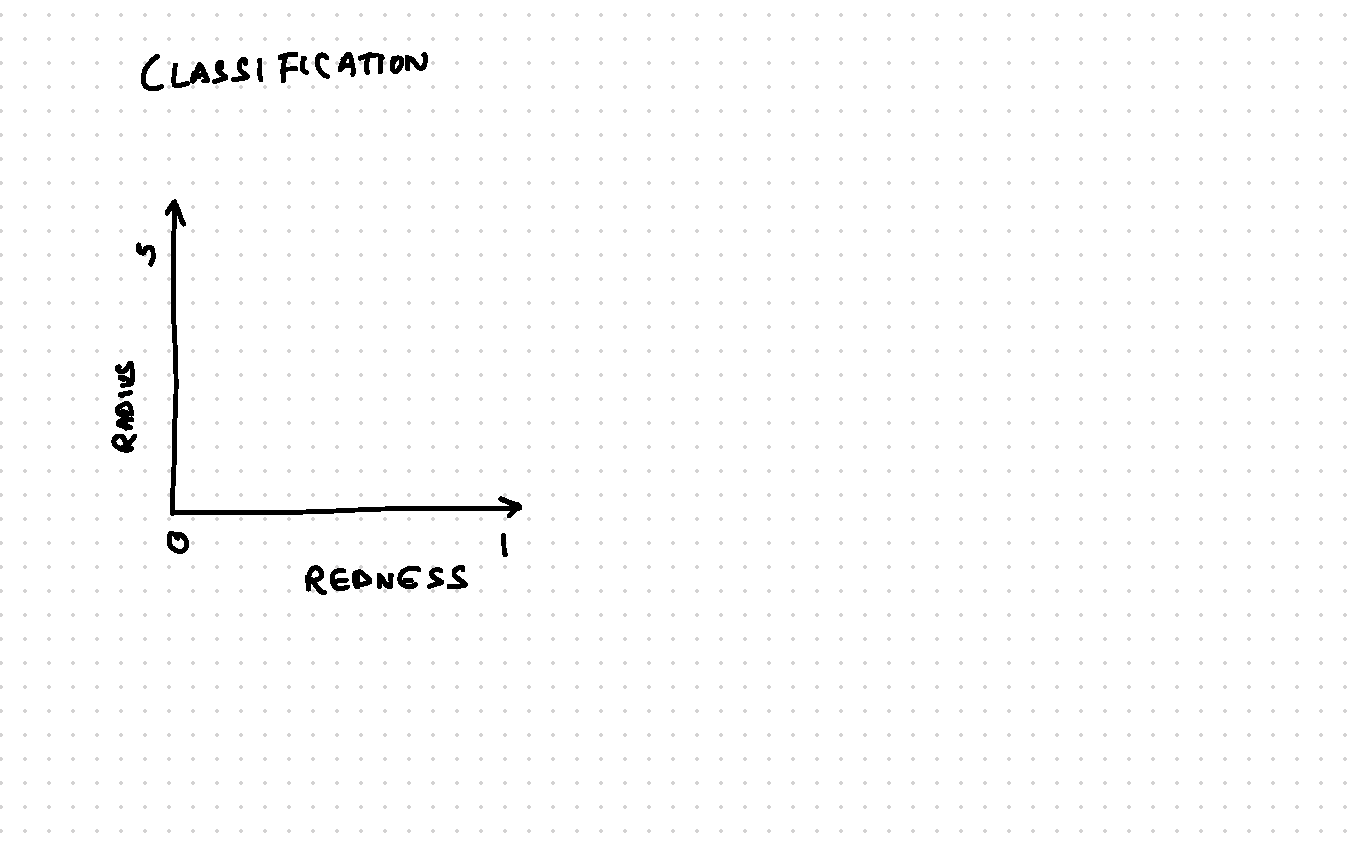
\includepdf[page=-]{knn/knn-intuition.pdf}
}

\begin{frame}{Important Considerations}
\begin{itemize}
\item<1-> What are the \textbf{features} that will be considered for data similarity?
\item<2-> What are the \textbf{total number} of features that are going to be taken into consideration?
\item<3-> What is the \textbf{distance metric} that will be used to calculate data similarity?
\item \checkmark \textbf{computational complexity} 
\end{itemize}
\end{frame}

\begin{frame}{KNN Algorithm}
\begin{itemize}
\item<1-> Keep the entire dataset: ${(x,y)}$
\item<2-> For a query vector $q$:
\begin{enumerate}
\item<3-> Find the k-closest data point(s) $x^*$
\item<4-> Predict $y^*$
\end{enumerate}
\end{itemize}
\end{frame}
  

\end{document}